\documentclass{article}\usepackage[]{graphicx}\usepackage[]{color}
%% maxwidth is the original width if it is less than linewidth
%% otherwise use linewidth (to make sure the graphics do not exceed the margin)
\makeatletter
\def\maxwidth{ %
  \ifdim\Gin@nat@width>\linewidth
    \linewidth
  \else
    \Gin@nat@width
  \fi
}
\makeatother

\definecolor{fgcolor}{rgb}{0.345, 0.345, 0.345}
\newcommand{\hlnum}[1]{\textcolor[rgb]{0.686,0.059,0.569}{#1}}%
\newcommand{\hlstr}[1]{\textcolor[rgb]{0.192,0.494,0.8}{#1}}%
\newcommand{\hlcom}[1]{\textcolor[rgb]{0.678,0.584,0.686}{\textit{#1}}}%
\newcommand{\hlopt}[1]{\textcolor[rgb]{0,0,0}{#1}}%
\newcommand{\hlstd}[1]{\textcolor[rgb]{0.345,0.345,0.345}{#1}}%
\newcommand{\hlkwa}[1]{\textcolor[rgb]{0.161,0.373,0.58}{\textbf{#1}}}%
\newcommand{\hlkwb}[1]{\textcolor[rgb]{0.69,0.353,0.396}{#1}}%
\newcommand{\hlkwc}[1]{\textcolor[rgb]{0.333,0.667,0.333}{#1}}%
\newcommand{\hlkwd}[1]{\textcolor[rgb]{0.737,0.353,0.396}{\textbf{#1}}}%

\usepackage{framed}
\makeatletter
\newenvironment{kframe}{%
 \def\at@end@of@kframe{}%
 \ifinner\ifhmode%
  \def\at@end@of@kframe{\end{minipage}}%
  \begin{minipage}{\columnwidth}%
 \fi\fi%
 \def\FrameCommand##1{\hskip\@totalleftmargin \hskip-\fboxsep
 \colorbox{shadecolor}{##1}\hskip-\fboxsep
     % There is no \\@totalrightmargin, so:
     \hskip-\linewidth \hskip-\@totalleftmargin \hskip\columnwidth}%
 \MakeFramed {\advance\hsize-\width
   \@totalleftmargin\z@ \linewidth\hsize
   \@setminipage}}%
 {\par\unskip\endMakeFramed%
 \at@end@of@kframe}
\makeatother

\definecolor{shadecolor}{rgb}{.97, .97, .97}
\definecolor{messagecolor}{rgb}{0, 0, 0}
\definecolor{warningcolor}{rgb}{1, 0, 1}
\definecolor{errorcolor}{rgb}{1, 0, 0}
\newenvironment{knitrout}{}{} % an empty environment to be redefined in TeX

\usepackage{alltt}
%\usepackage[margin=1in]{geometry}   % set up margins
\usepackage[vmargin=1in,hmargin=1in]{geometry}
\usepackage{tikz}
\usepackage{booktabs}

\usepackage[backend=bibtex]{biblatex}
\IfFileExists{upquote.sty}{\usepackage{upquote}}{}
\begin{document}

\title {Spatial Representation of Railway Congestion Reveals Motivation for a Multidimensional Pricing Model}
\author{Rebecca Brusky, Jace Crist, Davina Faimon, Jonah Williams, Joshua Wittenbach\\ Department of Mathematics\\ University of Nebraska at Omaha }

\maketitle



\begin{abstract}Currently, intermodal corporations have flat fee systems which do not incorporate a multidimensional pricing platform. One aspect which has yet to be utilized is freight capacity, which is difficult to conceptualize.  We plan to create a spatial visualization of the shipping traffic using data compiled from public sources.  We expect to find patterns of congestion on the rail systems between drayage points based on customer shipping requests. The results of this reproducible analysis can be used to assist in the forecasting of a multidimensional pricing model based on freight capacity coupled with customer parameters.  This congestion model will drive the possibilities for developing more sophisticated pricing systems in the future.
\end{abstract}

%\tableofcontents

\section{Introduction} Current models for pricing do not take advantage of data collected from intermodel websites. It is a flat fee system. The data collected can be mined for better more efficient methods.  Creating an automated process in which any intermodal company can use to leverage track network density into a pricing variable is the focus of this project. Using publicly available data, patterns in congestion through drayage nodes can be modeled and visualized as a proxy for analysis in order to understand customer demand.  This analysis provides a starting point for construction of tiered pricing models for intermodal corporations.

The process of intermodal shipping consists of a single mean of transportation from a customer to a drayage location where the cargo is then loaded onto any other mean of transportation.  The cargo is then picked up at a connecting drayage location and delivered to the receiving party or shipped internationally. However now our focus will be on the United States, and possible drayage with the intention of transportation across the country by the current most efficient way to transport commodities, railroad.

The visualization will consist of an underlayment of the trackage of the United States overlaid with shipping origination cities and railway drayage points. From the public information we've collected, we will show congestion patterns of shipping along railways in the United States.   \\

\section{Development Process} Originally, we were presented with a problem: Is there a way to create a dynamic pricing system that would improve on the current pricing system. We began considering different possibilities for data visualization and analysis of this intermodal shipping data such as railway traffic patterns and seasonal analysis. We found that the details of these orders necessary for more elaborate analysis proposed are not available publicly.  Nevertheless, the importance of drayage locations in the shipping process presented an opportunity for graph-based analysis considering the drayage node where the cargo enters and leaves the rail system.  The goal for our analysis is to understand the spatial traffic patterns through the drayage nodes.\\


\section{Artificial Data set} The first issue we have encountered is making private and confidential data public. We worked around the politics of the corporate world by mimicking the columns in which would be provided by any United States intermodal corporation. These are the steps we took in which would eliminate the need of private information.

First we must install and load the R libraries. \\


\begin{knitrout}
\definecolor{shadecolor}{rgb}{0.969, 0.969, 0.969}\color{fgcolor}\begin{kframe}
\begin{alltt}
\hlkwd{install.packages}\hlstd{(}\hlkwd{c}\hlstd{(}\hlstr{"maptools"}\hlstd{,} \hlstr{"data.table"}\hlstd{,} \hlstr{"ggmap"}\hlstd{,} \hlstr{"dplyr"}\hlstd{,} \hlstr{"RCurl"}\hlstd{,} \hlstr{"ggplot2"}\hlstd{,} \hlstr{"reshape2"}\hlstd{))}
\end{alltt}


{\ttfamily\noindent\itshape\color{messagecolor}{\#\# Installing packages into 'C:/Users/J/Documents/R/win-library/3.1'\\\#\# (as 'lib' is unspecified)}}

{\ttfamily\noindent\bfseries\color{errorcolor}{\#\# Error in contrib.url(repos, "{}source"{}): trying to use CRAN without setting a mirror}}\end{kframe}
\end{knitrout}

\begin{knitrout}
\definecolor{shadecolor}{rgb}{0.969, 0.969, 0.969}\color{fgcolor}\begin{kframe}
\begin{alltt}
\hlkwd{library}\hlstd{(RCurl)}
\end{alltt}


{\ttfamily\noindent\itshape\color{messagecolor}{\#\# Loading required package: bitops}}\begin{alltt}
\hlkwd{library}\hlstd{(reshape2)}
\hlkwd{library}\hlstd{(ggplot2)}
\hlkwd{library}\hlstd{(maptools)}
\end{alltt}


{\ttfamily\noindent\itshape\color{messagecolor}{\#\# Loading required package: sp\\\#\# Checking rgeos availability: FALSE\\\#\#\ \ 	Note: when rgeos is not available, polygon geometry 	computations in maptools depend on gpclib,\\\#\#\ \ 	which has a restricted licence. It is disabled by default;\\\#\#\ \ 	to enable gpclib, type gpclibPermit()}}\begin{alltt}
\hlkwd{library}\hlstd{(data.table)}
\hlkwd{library}\hlstd{(ggmap)}
\hlkwd{library}\hlstd{(dplyr)}
\end{alltt}


{\ttfamily\noindent\itshape\color{messagecolor}{\#\# \\\#\# Attaching package: 'dplyr'\\\#\# \\\#\# The following objects are masked from 'package:data.table':\\\#\# \\\#\#\ \ \ \  between, last\\\#\# \\\#\# The following object is masked from 'package:stats':\\\#\# \\\#\#\ \ \ \  filter\\\#\# \\\#\# The following objects are masked from 'package:base':\\\#\# \\\#\#\ \ \ \  intersect, setdiff, setequal, union}}\end{kframe}
\end{knitrout}


We have also created a source for all of our data to be accessed by the public. We will call some of that data. This will help us produce an artificial data set. \\

\begin{knitrout}
\definecolor{shadecolor}{rgb}{0.969, 0.969, 0.969}\color{fgcolor}\begin{kframe}
\begin{alltt}
\hlstd{data1} \hlkwb{<-} \hlkwd{getURL}\hlstd{(}
  \hlstr{'https://raw.githubusercontent.com/Jwcrist/Group-2/master/Data/origin_lat_long3.csv'}\hlstd{,}
  \hlkwc{ssl.verifypeer}\hlstd{=}\hlnum{0L}\hlstd{,} \hlkwc{followlocation}\hlstd{=}\hlnum{1L}\hlstd{)}
\hlstd{origin} \hlkwb{<-} \hlkwd{read.csv}\hlstd{(}\hlkwc{text}\hlstd{=data1)}
\hlstd{origin}
\end{alltt}
\begin{verbatim}
##                              X        lon      lat
## 1               FRANKLIN -  TN  -86.86889 35.92506
## 2                CONCORD -  CA -122.03107 37.97798
## 3                  TYLER -  TX  -95.30106 32.35126
## 4                PHOENIX -  AZ -112.07404 33.44838
## 5              NORTHLAKE -  IL  -87.89562 41.91725
## 6            MISSISSAUGA -  ON  -79.64412 43.58905
## 7                 ORANGE -  CA -117.85311 33.78779
## 8                BUFFALO -  NY  -78.87837 42.88645
## 9             LAS CRUCES -  NM -106.76365 32.31994
## 10              LAKELAND -  FL  -81.94980 28.03947
## 11               SEATTLE -  WA -122.33207 47.60621
## 12                BURIEN -  WA -122.34679 47.47038
## 13            GRANDVILLE -  MI  -85.76309 42.90975
## 14      ENGLEWOOD CLIFFS -  NJ  -73.95236 40.88538
## 15             ROSEVILLE -  MN  -93.15661 45.00608
## 16                 OMAHA -  NE  -95.99799 41.25236
## 17           CHATTANOOGA -  TN  -85.30968 35.04563
## 18            NAPERVILLE -  IL  -88.16188 41.74607
## 19            FARMINGTON -  NY  -77.32194 42.98083
## 20             RIVERVIEW -  FL  -82.32648 27.86614
## 21             STOUGHTON -  WI  -89.21789 42.91695
## 22              BUCHANAN -  MI  -86.36112 41.82727
## 23               MEMPHIS -  TN  -90.04898 35.14953
## 24                JEROME -  ID -114.51865 42.72407
## 25                SKOKIE -  IL  -87.74162 42.03240
## 26           WESTERVILLE -  OH  -82.92907 40.12617
## 27     ELK GROVE VILLAGE -  IL  -87.97035 42.00392
## 28                  RENO -  NV -119.81380 39.52963
## 29              GLENSIDE -  PA  -75.15279 40.09991
## 30                FRISCO -  TX  -96.82361 33.15067
## 31          MURFREESBORO -  TN  -86.39027 35.84562
## 32            PORTSMOUTH -  NH  -70.76255 43.07176
## 33             ROCHESTER -  NY  -77.61092 43.16103
## 34               SEAFORD -  DE  -75.61104 38.64123
## 35               CORDOVA -  TN  -89.76155 35.15983
## 36            ST LAURENT -  PQ  -73.74976 45.49856
## 37      BOULDER JUNCTION -  WI  -89.64410 46.11304
## 38             VAN BUREN -  AR  -94.34827 35.43676
## 39               LEBANON -  PA  -76.41135 40.34093
## 40                EXETER -  NH  -70.94775 42.98143
## 41            EARTH CITY -  MO  -90.46675 38.76992
## 42               LA PINE -  OR -121.50364 43.67040
## 43                DENVER -  CO -104.98472 39.73757
## 44             BLUE BELL -  PA  -75.26629 40.15233
## 45                TACOMA -  WA -122.44429 47.25288
## 46               HOLLAND -  OH  -83.71160 41.62172
## 47            COOKEVILLE -  TN  -85.50164 36.16284
## 48          EAST DUBUQUE -  IL  -90.64291 42.49223
## 49              SECAUCUS -  NJ  -74.05653 40.78955
## 50        SALT LAKE CITY -  UT -111.89105 40.76078
## 51               CHICAGO -  IL  -87.62980 41.87811
## 52              PORTLAND -  OR -122.67621 45.52345
## 53             KENNEWICK -  WA -119.13723 46.21125
## 54                FRESNO -  CA -119.77259 36.74684
## 55            VALPARAISO -  IN  -87.06114 41.47309
## 56                  ROME -  GA  -85.16467 34.25704
## 57           BOLINGBROOK -  IL  -88.06840 41.69864
## 58          JACKSONVILLE -  FL  -81.65565 30.33218
## 59            BURLINGTON -  NJ  -74.86489 40.07122
## 60             ANN ARBOR -  MI  -83.74304 42.28083
## 61             FRANKFORT -  IL  -87.84866 41.49587
## 62      GLENDALE HEIGHTS -  IL  -88.07174 41.91031
## 63               EVERETT -  WA -122.20208 47.97898
## 64               MONDOVI -  WI  -91.67099 44.56774
## 65              DAVIDSON -  NC  -80.84868 35.49930
## 66             WOODRIDGE -  IL  -88.05034 41.74697
## 67             ST HUBERT -  PQ  -73.40651 45.49833
## 68             PAULSBORO -  NJ  -75.24046 39.83039
## 69          EDEN PRAIRIE -  MN  -93.47079 44.85469
## 70            AUBURNDALE -  FL  -81.78869 28.06530
## 71           SAINT LOUIS -  MO  -90.19940 38.62700
## 72             PAPILLION -  NE  -96.04224 41.15444
## 73                ITASCA -  IL  -88.00729 41.97503
## 74          INDIANAPOLIS -  IN  -86.15807 39.76840
## 75                IRVING -  TX  -96.94889 32.81402
## 76                PALMER -  MA  -72.32869 42.15841
## 77             FAIRFIELD -  NJ  -74.30600 40.88374
## 78            CINCINNATI -  OH  -84.51202 39.10312
## 79              VINELAND -  NJ  -75.02596 39.48638
## 80            WILMINGTON -  NC  -77.94471 34.22573
## 81              CRANFORD -  NJ  -74.29959 40.65842
## 82              BROOKLYN -  NY  -73.94416 40.67818
## 83             ROCHESTER -  PA  -80.28645 40.70229
## 84                  YORK -  SC  -81.24202 34.99430
## 85               HOUSTON -  TX  -95.36939 29.76019
## 86            GREENSBORO -  NC  -79.79198 36.07264
## 87             BOUNTIFUL -  UT -111.88077 40.88939
## 88            ALPHARETTA -  GA  -84.29409 34.07538
## 89                LENEXA -  KS  -94.73357 38.95362
## 90        GRAND JUNCTION -  CO -108.55065 39.06387
## 91            BOCA RATON -  FL  -80.12893 26.36831
## 92        HENDERSONVILLE -  TN  -86.62000 36.30477
## 93            NORTHFIELD -  IL  -87.78090 42.09975
## 94            FORT SMITH -  AR  -94.39855 35.38592
## 95              KINGSTON -  WA -122.49819 47.79871
## 96            WOOD RIVER -  IL  -90.09761 38.86116
## 97               AMHERST -  NY  -78.79142 42.97561
## 98           TINLEY PARK -  IL  -87.79329 41.57314
## 99              FLORENCE -  KY  -84.62661 38.99895
## 100            LA MIRADA -  CA -118.01201 33.91724
## 101              SHAWNEE -  KS  -94.71519 39.02285
## 102             MONTREAL -  PQ  -73.55399 45.50867
## 103           FORT MYERS -  FL  -81.87231 26.64063
## 104             LIMERICK -  PA  -75.52212 40.23093
## 105          LOS ANGELES -  CA -118.24368 34.05223
## 106     CITY OF COMMERCE -  CA -118.15979 34.00057
## 107               BOSTON -  MA  -71.05977 42.35843
## 108         CAROL STREAM -  IL  -88.13479 41.91253
## 109            GREEN BAY -  WI  -88.01983 44.51916
## 110          LAKE ZURICH -  IL  -88.09341 42.19697
## 111               CORONA -  CA -117.56644 33.87529
## 112      ROLLING MEADOWS -  IL  -88.01313 42.08419
## 113           WENTZVILLE -  MO  -90.85291 38.81144
## 114         CEDAR RAPIDS -  IA  -91.66562 41.97788
## 115             OAK LAWN -  IL  -87.74795 41.71998
## 116             GIBSONIA -  PA  -79.97033 40.63006
## 117            GREENWOOD -  IN  -86.10665 39.61366
## 118             MURRIETA -  CA -117.21392 33.55391
## 119           PITTSBURGH -  PA  -79.99589 40.44062
## 120         SANTA MONICA -  CA -118.49119 34.01945
## 121                 TROY -  MO  -90.98070 38.97949
## 122            LANGHORNE -  PA  -74.92267 40.17455
## 123          UNION GROVE -  WI  -88.05147 42.68807
## 124            SAN DIEGO -  CA -117.16108 32.71574
## 125         MELROSE PARK -  IL  -87.85673 41.90059
## 126            SANTA ANA -  CA -117.86783 33.74557
## 127           CHATSWORTH -  CA -118.61481 34.25064
## 128               CICERO -  IL  -87.75394 41.84559
## 129            GLADSTONE -  MO  -94.55468 39.20389
## 130          PEARL RIVER -  NY  -74.02181 41.05899
## 131               TIGARD -  OR -122.77149 45.43123
## 132     RANCHO CUCAMONGA -  CA -117.59311 34.10640
## 133             MARIETTA -  GA  -84.54993 33.95260
## 134          WESTMINSTER -  MD  -76.99581 39.57538
## 135              ANAHEIM -  CA -117.91450 33.83529
## 136          SIOUX FALLS -  SD  -96.73110 43.54460
## 137          LAKE FOREST -  IL  -87.84063 42.25863
## 138                 KENT -  OH  -81.35789 41.15367
## 139      DEERFIELD BEACH -  FL  -80.09977 26.31841
## 140      WEST SACRAMENTO -  CA -121.53023 38.58046
## 141            MANITOWOC -  WI  -87.65758 44.08861
## 142              MEDFORD -  OR -122.87559 42.32652
## 143         SOLANA BEACH -  CA -117.27115 32.99115
## 144        OVERLAND PARK -  KS  -94.67079 38.98223
## 145               IXONIA -  WI  -88.59732 43.14389
## 146            GRAPEVINE -  TX  -97.07807 32.93429
## 147             DEFIANCE -  OH  -84.35578 41.28449
## 148          WATSONVILLE -  CA -121.75689 36.91023
## 149     ROYAL PALM BEACH -  FL  -80.23060 26.70840
## 150        SANTA CLARITA -  CA -118.54259 34.39166
## 151               WAUKEE -  IA  -93.88558 41.61199
## 152        LAGUNA NIGUEL -  CA -117.70755 33.52253
## 153       MOUNT PLEASANT -  SC  -79.82843 32.83232
## 154               DALLAS -  TX  -96.80045 32.78014
## 155                 AVON -  MA  -71.04116 42.13066
## 156               OLATHE -  KS  -94.81913 38.88140
## 157             NORCROSS -  GA  -84.21353 33.94121
## 158          MINNEAPOLIS -  MN  -93.26667 44.98333
## 159              REDDING -  CA -122.39168 40.58654
## 160           BURLINGTON -  ON  -79.79903 43.32552
## 161            MANSFIELD -  TX  -97.14168 32.56319
## 162              BEDFORD -  TX  -97.14307 32.84402
## 163        BUFFALO GROVE -  IL  -87.96313 42.16628
## 164             COOS BAY -  OR -124.21789 43.36650
## 165              LASALLE -  QC  -73.63480 45.43063
## 166            KNOXVILLE -  TN  -83.92074 35.96064
## 167         ORMOND BEACH -  FL  -81.05589 29.28581
## 168             LAKEWOOD -  OH  -81.79819 41.48199
## 169               AURORA -  CO -104.83192 39.72943
## 170            LANCASTER -  PA  -76.30551 40.03788
## 171                CRETE -  IL  -87.63143 41.44448
## 172              CONCORD -  NC  -80.57951 35.40875
## 173             STONEHAM -  MA  -71.09997 42.48025
## 174            MARQUETTE -  MI  -87.39560 46.54758
## 175           ROUND ROCK -  TX  -97.67890 30.50826
## 176          LAKE OSWEGO -  OR -122.67065 45.42067
## 177             NEW YORK -  NY  -74.00594 40.71278
## 178          BRIDGEWATER -  MA  -70.97505 41.99035
## 179         MULLICA HILL -  NJ  -75.22407 39.73928
## 180              CALGARY -  AB -114.05810 51.04532
## 181            CHARLOTTE -  NC  -80.84313 35.22709
## 182      MENOMONEE FALLS -  WI  -88.11731 43.17890
## 183             COLUMBUS -  OH  -82.99879 39.96118
## 184             STREATOR -  IL  -88.83535 41.12087
## 185            BALTIMORE -  MD  -76.61219 39.29038
## 186          PUNTA GORDA -  FL  -82.04537 26.92978
## 187                MIAMI -  FL  -80.20404 25.78910
## 188             LAKEWOOD -  NJ  -74.20970 40.08213
## 189           BROOKFIELD -  WI  -88.10648 43.06057
## 190             PITCAIRN -  PA  -79.77810 40.40312
## 191           ROMEOVILLE -  IL  -88.08951 41.64753
## 192            STUTTGART -  AR  -91.55263 34.50037
## 193              WARWICK -  RI  -71.41617 41.70010
## 194           CASEYVILLE -  IL  -90.02566 38.63672
## 195            LIVERMORE -  CA -121.76801 37.68187
## 196              LOMBARD -  IL  -88.00784 41.88003
## 197              JAMAICA -  NY  -73.78897 40.70268
## 198                 LODI -  CA -121.27222 38.13415
## 199             BELLEVUE -  WA -122.20068 47.61038
## 200               CONLEY -  GA  -84.34222 33.64028
## 201              LINWOOD -  NJ  -74.57516 39.33984
## 202              EL PASO -  TX -106.44246 31.77758
## 203             EDINBORO -  PA  -80.13172 41.87422
## 204              SUNCOOK -  NH  -71.45312 43.13064
## 205       PEMBROKE PINES -  FL  -80.29626 26.00776
## 206               HUMBLE -  TX  -95.26216 29.99883
## 207           MONTEBELLO -  CA -118.11375 34.01651
## 208            BRADENTON -  FL  -82.57482 27.49893
## 209          KANSAS CITY -  MO  -94.57857 39.09973
## 210           LOUISVILLE -  CO -105.13193 39.97776
## 211               CANTON -  OH  -81.37845 40.79895
## 212            ESSINGTON -  PA  -75.29700 39.86215
## 213                NILES -  IL  -87.80284 42.01892
## 214             TORRANCE -  CA -118.34063 33.83585
## 215              BOZEMAN -  MT -111.04722 45.67778
## 216          SAINT CLOUD -  MN  -94.16324 45.55795
## 217              CLINTON -  IL  -88.96453 40.15365
## 218             LOCKWOOD -  MO  -93.95327 37.38560
## 219              PRESTON -  MD  -75.90994 38.71262
## 220           PLEASANTON -  CA -121.87468 37.66243
## 221              PORTAGE -  OH  -83.65077 41.32672
## 222 LA CANADA FLINTRIDGE -  CA -118.20003 34.20682
## 223         FAYETTEVILLE -  AR  -94.15743 36.06258
## 224        COTEAU-DU-LAC -  QC  -74.17468 45.29163
## 225                EAGAN -  MN  -93.16689 44.80413
## 226            NEW LENOX -  IL  -87.96561 41.51198
## 227  INVER GROVE HEIGHTS -  MN  -93.04272 44.84802
## 228         PFLUGERVILLE -  TX  -97.62000 30.43937
## 229           MANDEVILLE -  LA  -90.06563 30.35825
## 230     CANAL WINCHESTER -  OH  -82.81236 39.84666
## 231          WILSONVILLE -  OR -122.77371 45.29984
## 232              TORONTO -  ON  -79.38318 43.65323
## 233              HOLLAND -  MI  -86.10893 42.78752
## 234            MILWAUKIE -  OR -122.63926 45.44623
## 235         SOUTHBOROUGH -  MA  -71.52451 42.30565
## 236               MOKENA -  IL  -87.88922 41.52614
## 237                ELGIN -  IL  -88.28333 42.03333
## 238              ALTOONA -  PA  -78.39474 40.51868
## 239    HUNTINGDON VALLEY -  PA  -75.07280 40.13799
## 240            MCDONOUGH -  GA  -84.14686 33.44734
## 241             LITHONIA -  GA  -84.10519 33.71233
## 242             BARTLETT -  TN  -89.87398 35.20453
## 243             CROSSETT -  AR  -91.96124 33.12818
## 244           BROOKFIELD -  IL  -87.85173 41.82392
## 245          WILLOWBROOK -  IL  -87.93589 41.76975
## 246             BELLEVUE -  NE  -95.93417 41.15861
## 247                 BREA -  CA -117.90006 33.91668
## 248               POMONA -  CA -117.74999 34.05510
## 249      NORTH HOLLYWOOD -  CA -118.38126 34.18704
## 250           SOUTHFIELD -  MI  -83.22187 42.47337
## 251            CAMARILLO -  CA -119.03760 34.21639
## 252             ROCKFORD -  IL  -89.09400 42.27113
## 253            ROSEMOUNT -  MN  -93.12577 44.73941
## 254               SEWELL -  NJ  -75.14419 39.76622
## 255          CHERRY HILL -  NJ  -75.02463 39.92681
## 256         PHILADELPHIA -  PA  -75.16379 39.95233
## 257             PLYMOUTH -  MA  -70.66726 41.95845
## 258         WEST CHICAGO -  IL  -88.20396 41.88475
## 259               DAYTON -  OH  -84.19161 39.75895
## 260          LITTLE ROCK -  AR  -92.28959 34.74648
## 261           DOYLESTOWN -  PA  -75.12989 40.31011
## 262       WEST FRANKFORT -  IL  -88.92336 37.89860
## 263           WEST FARGO -  ND  -96.89991 46.87695
## 264         COLLIERVILLE -  TN  -89.66453 35.04204
## 265              NORWALK -  CA -118.08173 33.90224
## 266               BUFORD -  GA  -84.00435 34.12066
## 267              SISTERS -  OR -121.54921 44.29095
## 268           YOUNGSTOWN -  OH  -80.64952 41.09978
## 269       MARINA DEL REY -  CA -118.45174 33.98029
## 270            VANCOUVER -  WA -122.66149 45.63873
## 271             WINNIPEG -  MB  -97.13749 49.89975
## 272              BURBANK -  IL  -87.76074 41.74676
## 273               AUSTIN -  TX  -97.74306 30.26715
## 274        DOWNERS GROVE -  IL  -88.01117 41.80892
## 275              WOOSTER -  OH  -81.93514 40.80506
## 276              BRANDON -  FL  -82.28592 27.93780
## 277               URBANA -  OH  -83.75243 40.10839
## 278       FOUNTAIN HILLS -  AZ -111.72000 33.60000
## 279           CORAOPOLIS -  PA  -80.16672 40.51840
## 280               WALNUT -  CA -117.86534 34.02029
## 281           BIRMINGHAM -  AL  -86.80249 33.52066
## 282          SUGAR GROVE -  IL  -88.44369 41.76142
## 283             LANSDALE -  PA  -75.28379 40.24150
## 284                OLNEY -  IL  -88.08532 38.73088
## 285               EULESS -  TX  -97.08195 32.83707
## 286              VISALIA -  CA -119.29206 36.33023
## 287             MATTHEWS -  NC  -80.72368 35.11681
## 288               SURREY -  BC -122.85000 49.18333
## 289              OSCEOLA -  IN  -86.07584 41.66505
## 290              OSHKOSH -  WI  -88.54261 44.02471
## 291              VENTURA -  CA -119.22903 34.27465
## 292           WOODBRIDGE -  NJ  -74.28460 40.55760
## 293          PICO RIVERA -  CA -118.09673 33.98307
## 294                COCOA -  FL  -80.74200 28.38612
## 295           LAKE ORION -  MI  -83.23966 42.78448
## 296            WOOD DALE -  IL  -87.97896 41.96336
## 297                LISLE -  IL  -88.07479 41.80114
## 298             WOODBURY -  NY  -73.46762 40.82565
## 299                 NIXA -  MO  -93.29435 37.04339
## 300              BATAVIA -  IL  -88.31257 41.85003
## 301            WILKINSON -  IN  -85.60886 39.88588
## 302            WAKEFIELD -  RI  -71.50145 41.43732
## 303             FLORENCE -  SC  -79.76256 34.19543
## 304           SCOTTSDALE -  AZ -111.92605 33.49417
## 305     SANTA FE SPRINGS -  CA -118.08535 33.94724
## 306           LONG BEACH -  CA -118.19374 33.77005
## 307            SAN RAMON -  CA -121.97802 37.77993
## 308             HAMILTON -  MT -114.15482 46.24714
## 309               RACINE -  WI  -87.78285 42.72613
## 310        WEST COLUMBIA -  SC  -81.07398 33.99349
## 311                HURST -  TX  -97.17057 32.82346
## 312               QUINCY -  IL  -91.40987 39.93560
## 313         NORTH BERGEN -  NJ  -74.01208 40.80427
## 314          SPRINGFIELD -  MA  -72.58981 42.10148
## 315              SUNRISE -  FL  -80.25660 26.16697
## 316             OAKHURST -  CA -119.64932 37.32800
## 317             RINGWOOD -  NJ  -74.24543 41.11343
## 318           CENTENNIAL -  CO -104.87717 39.58075
## 319      MENDOTA HEIGHTS -  MN  -93.13827 44.88358
## 320              COMPTON -  CA -118.22007 33.89585
## 321              OAKLAND -  CA -122.27111 37.80436
## 322              ANTIOCH -  IL  -88.09564 42.47724
## 323           FORT WAYNE -  IN  -85.13935 41.07927
## 324               AUBURN -  WA -122.22845 47.30732
## 325           WOODBRIDGE -  ON  -79.61298 43.78905
## 326        FRANKLIN PARK -  IL  -87.87952 41.93485
## 327            RIVERSIDE -  CA -117.39616 33.95335
## 328         MORTON GROVE -  IL  -87.78256 42.04059
## 329            LA PUENTE -  CA -117.94951 34.02001
## 330          COLD SPRING -  KY  -84.43994 39.02173
## 331            ELIZABETH -  NJ  -74.21070 40.66399
## 332           PLAINFIELD -  IN  -86.39944 39.70421
## 333            TONTITOWN -  AR  -94.23354 36.17786
## 334                 AYER -  MA  -71.58991 42.56119
## 335            CARLSTADT -  NJ  -74.09070 40.84038
## 336           LEWISVILLE -  TX  -96.99417 33.04623
## 337            RIVERSIDE -  RI  -71.36478 41.76732
## 338         HACKETTSTOWN -  NJ  -74.82906 40.85399
## 339           CARROLLTON -  TX  -96.88996 32.97564
## 340              WHEATON -  IL  -88.10701 41.86614
## 341               EASTON -  PA  -75.22073 40.68843
## 342             STILWELL -  KS  -94.65921 38.76729
## 343         MOUNT LAUREL -  NJ  -74.89100 39.93400
## 344               LAREDO -  TX  -99.48032 27.53057
## 345          BENSENVILLE -  IL  -87.94007 41.95503
## 346               CALERA -  AL  -86.75360 33.10290
## 347          OLD HICKORY -  TN  -86.64777 36.25749
## 348            GLEN ROCK -  NJ  -74.13292 40.96288
## 349               DUBLIN -  CA -121.93579 37.70215
## 350              POTSDAM -  NY  -74.98131 44.66978
## 351               NEWNAN -  GA  -84.79966 33.38067
## 352            GLADSTONE -  OR -122.59481 45.38068
## 353             CARLISLE -  PA  -77.19500 40.20250
## 354            MILWAUKEE -  WI  -87.90647 43.03890
## 355           SACRAMENTO -  CA -121.49440 38.58157
## 356             RICHMOND -  VA  -77.43605 37.54072
## 357          JERSEY CITY -  NJ  -74.07764 40.72816
## 358           LOUISVILLE -  KY  -85.75846 38.25266
## 359              OAKDALE -  MN  -92.96494 44.96302
## 360              HOUSTON -  AL  -87.25807 34.14149
## 361               IRVINE -  CA -117.79469 33.68395
## 362              FINDLAY -  OH  -83.64993 41.04422
## 363            ALTAMAHAW -  NC  -79.50725 36.18430
## 364              MAYNARD -  MA  -71.44951 42.43349
## 365               LATHAM -  NY  -73.75889 42.74694
## 366             BROOMALL -  PA  -75.35472 39.97167
## 367                  LEE -  NH  -71.01201 43.12224
## 368           ROUND LAKE -  NY  -73.78984 42.93869
## 369             RED BANK -  NJ  -74.06431 40.34705
## 370             MONTVALE -  NJ  -74.02292 41.04676
## 371        WHITMORE LAKE -  MI  -83.74383 42.43948
## 372            STRAFFORD -  MO  -93.11713 37.26838
## 373              MIRAMAR -  FL  -80.30356 25.98608
## 374           VINCENTOWN -  NJ  -74.74861 39.93389
## 375        MONTEREY PARK -  CA -118.12285 34.06251
## 376            LAS VEGAS -  NV -115.13983 36.16994
## 377             HINSDALE -  IL  -87.93701 41.80086
## 378               CARMEL -  IN  -86.11804 39.97837
## 379               TAYLOR -  MI  -83.26965 42.24087
## 380          ROCK ISLAND -  IL  -90.57875 41.50948
## 381              MALVERN -  AR  -92.81295 34.36231
## 382            ROBESONIA -  PA  -76.13439 40.35176
## 383               NEWTON -  MA  -71.20922 42.33704
## 384           RUTHERFORD -  NJ  -74.10681 40.82649
## 385             OAKVILLE -  ON  -79.68767 43.46752
## 386          GAINESVILLE -  GA  -83.82407 34.29788
## 387               TUCKER -  GA  -84.21714 33.85455
## 388               SPRING -  TX  -95.41716 30.07994
## 389      NORTH BRUNSWICK -  NJ  -74.47667 40.45252
## 390          LINCOLNWOOD -  IL  -87.73006 42.00448
## 391              WINDSOR -  CO -104.90136 40.47748
## 392            HAUPPAUGE -  NY  -73.20261 40.82565
## 393            ROYAL OAK -  MI  -83.14465 42.48948
## 394              GILBERT -  AZ -111.78903 33.35283
## 395            POTTSTOWN -  PA  -75.64963 40.24537
## 396                 NOVI -  MI  -83.47549 42.48059
## 397     CITY OF INDUSTRY -  CA -117.95868 34.01973
## 398       SAN BERNARDINO -  CA -117.28977 34.10834
## 399             DEFIANCE -  MO  -90.77818 38.63250
## 400                TAMPA -  FL  -82.45718 27.95058
## 401              LINWOOD -  NJ  -74.57516 39.33984
## 402              EL PASO -  TX -106.44246 31.77758
## 403             EDINBORO -  PA  -80.13172 41.87422
## 404              SUNCOOK -  NH  -71.45312 43.13064
## 405       PEMBROKE PINES -  FL  -80.29626 26.00776
## 406               HUMBLE -  TX  -95.26216 29.99883
## 407           MONTEBELLO -  CA -118.11375 34.01651
## 408            BRADENTON -  FL  -82.57482 27.49893
## 409          KANSAS CITY -  MO  -94.57857 39.09973
## 410           LOUISVILLE -  CO -105.13193 39.97776
## 411               CANTON -  OH  -81.37845 40.79895
## 412            ESSINGTON -  PA  -75.29700 39.86215
## 413                NILES -  IL  -87.80284 42.01892
## 414             TORRANCE -  CA -118.34063 33.83585
## 415              BOZEMAN -  MT -111.04722 45.67778
## 416          SAINT CLOUD -  MN  -94.16324 45.55795
## 417              CLINTON -  IL  -88.96453 40.15365
## 418             LOCKWOOD -  MO  -93.95327 37.38560
## 419              PRESTON -  MD  -75.90994 38.71262
## 420           PLEASANTON -  CA -121.87468 37.66243
## 421              PORTAGE -  OH  -83.65077 41.32672
## 422 LA CANADA FLINTRIDGE -  CA -118.20003 34.20682
## 423         FAYETTEVILLE -  AR  -94.15743 36.06258
## 424        COTEAU-DU-LAC -  QC  -74.17468 45.29163
## 425                EAGAN -  MN  -93.16689 44.80413
## 426            NEW LENOX -  IL  -87.96561 41.51198
## 427  INVER GROVE HEIGHTS -  MN  -93.04272 44.84802
## 428         PFLUGERVILLE -  TX  -97.62000 30.43937
## 429           MANDEVILLE -  LA  -90.06563 30.35825
## 430     CANAL WINCHESTER -  OH  -82.81236 39.84666
## 431          WILSONVILLE -  OR -122.77371 45.29984
## 432              TORONTO -  ON  -79.38318 43.65323
## 433              HOLLAND -  MI  -86.10893 42.78752
## 434            MILWAUKIE -  OR -122.63926 45.44623
## 435         SOUTHBOROUGH -  MA  -71.52451 42.30565
## 436               MOKENA -  IL  -87.88922 41.52614
## 437                ELGIN -  IL  -88.28333 42.03333
## 438              ALTOONA -  PA  -78.39474 40.51868
## 439    HUNTINGDON VALLEY -  PA  -75.07280 40.13799
## 440            MCDONOUGH -  GA  -84.14686 33.44734
## 441             LITHONIA -  GA  -84.10519 33.71233
## 442             BARTLETT -  TN  -89.87398 35.20453
## 443             CROSSETT -  AR  -91.96124 33.12818
## 444           BROOKFIELD -  IL  -87.85173 41.82392
## 445          WILLOWBROOK -  IL  -87.93589 41.76975
## 446             BELLEVUE -  NE  -95.93417 41.15861
## 447                 BREA -  CA -117.90006 33.91668
## 448               POMONA -  CA -117.74999 34.05510
## 449      NORTH HOLLYWOOD -  CA -118.38126 34.18704
## 450           SOUTHFIELD -  MI  -83.22187 42.47337
## 451            CAMARILLO -  CA -119.03760 34.21639
## 452             ROCKFORD -  IL  -89.09400 42.27113
## 453            ROSEMOUNT -  MN  -93.12577 44.73941
## 454               SEWELL -  NJ  -75.14419 39.76622
## 455          CHERRY HILL -  NJ  -75.02463 39.92681
## 456         PHILADELPHIA -  PA  -75.16379 39.95233
## 457             PLYMOUTH -  MA  -70.66726 41.95845
## 458         WEST CHICAGO -  IL  -88.20396 41.88475
## 459               DAYTON -  OH  -84.19161 39.75895
## 460          LITTLE ROCK -  AR  -92.28959 34.74648
## 461           DOYLESTOWN -  PA  -75.12989 40.31011
## 462       WEST FRANKFORT -  IL  -88.92336 37.89860
## 463           WEST FARGO -  ND  -96.89991 46.87695
## 464         COLLIERVILLE -  TN  -89.66453 35.04204
## 465              NORWALK -  CA -118.08173 33.90224
## 466               BUFORD -  GA  -84.00435 34.12066
## 467              SISTERS -  OR -121.54921 44.29095
## 468           YOUNGSTOWN -  OH  -80.64952 41.09978
## 469       MARINA DEL REY -  CA -118.45174 33.98029
## 470            VANCOUVER -  WA -122.66149 45.63873
## 471             WINNIPEG -  MB  -97.13749 49.89975
## 472              BURBANK -  IL  -87.76074 41.74676
## 473               AUSTIN -  TX  -97.74306 30.26715
## 474        DOWNERS GROVE -  IL  -88.01117 41.80892
## 475              WOOSTER -  OH  -81.93514 40.80506
## 476              BRANDON -  FL  -82.28592 27.93780
## 477               URBANA -  OH  -83.75243 40.10839
## 478       FOUNTAIN HILLS -  AZ -111.72000 33.60000
## 479           CORAOPOLIS -  PA  -80.16672 40.51840
## 480               WALNUT -  CA -117.86534 34.02029
## 481           BIRMINGHAM -  AL  -86.80249 33.52066
## 482          SUGAR GROVE -  IL  -88.44369 41.76142
## 483             LANSDALE -  PA  -75.28379 40.24150
## 484                OLNEY -  IL  -88.08532 38.73088
## 485               EULESS -  TX  -97.08195 32.83707
## 486              VISALIA -  CA -119.29206 36.33023
## 487             MATTHEWS -  NC  -80.72368 35.11681
## 488               SURREY -  BC -122.85000 49.18333
## 489              OSCEOLA -  IN  -86.07584 41.66505
## 490              OSHKOSH -  WI  -88.54261 44.02471
## 491              VENTURA -  CA -119.22903 34.27465
## 492           WOODBRIDGE -  NJ  -74.28460 40.55760
## 493          PICO RIVERA -  CA -118.09673 33.98307
## 494                COCOA -  FL  -80.74200 28.38612
## 495           LAKE ORION -  MI  -83.23966 42.78448
## 496            WOOD DALE -  IL  -87.97896 41.96336
## 497                LISLE -  IL  -88.07479 41.80114
## 498             WOODBURY -  NY  -73.46762 40.82565
## 499                 NIXA -  MO  -93.29435 37.04339
## 500              BATAVIA -  IL  -88.31257 41.85003
## 501            WILKINSON -  IN  -85.60886 39.88588
## 502            WAKEFIELD -  RI  -71.50145 41.43732
## 503             FLORENCE -  SC  -79.76256 34.19543
## 504           SCOTTSDALE -  AZ -111.92605 33.49417
## 505     SANTA FE SPRINGS -  CA -118.08535 33.94724
## 506           LONG BEACH -  CA -118.19374 33.77005
## 507            SAN RAMON -  CA -121.97802 37.77993
## 508             HAMILTON -  MT -114.15482 46.24714
## 509               RACINE -  WI  -87.78285 42.72613
## 510        WEST COLUMBIA -  SC  -81.07398 33.99349
## 511                HURST -  TX  -97.17057 32.82346
## 512               QUINCY -  IL  -91.40987 39.93560
## 513         NORTH BERGEN -  NJ  -74.01208 40.80427
## 514          SPRINGFIELD -  MA  -72.58981 42.10148
## 515              SUNRISE -  FL  -80.25660 26.16697
## 516             OAKHURST -  CA -119.64932 37.32800
## 517             RINGWOOD -  NJ  -74.24543 41.11343
## 518           CENTENNIAL -  CO -104.87717 39.58075
## 519      MENDOTA HEIGHTS -  MN  -93.13827 44.88358
## 520              COMPTON -  CA -118.22007 33.89585
## 521              OAKLAND -  CA -122.27111 37.80436
## 522              ANTIOCH -  IL  -88.09564 42.47724
## 523           FORT WAYNE -  IN  -85.13935 41.07927
## 524               AUBURN -  WA -122.22845 47.30732
## 525           WOODBRIDGE -  ON  -79.61298 43.78905
## 526        FRANKLIN PARK -  IL  -87.87952 41.93485
## 527            RIVERSIDE -  CA -117.39616 33.95335
## 528         MORTON GROVE -  IL  -87.78256 42.04059
## 529            LA PUENTE -  CA -117.94951 34.02001
## 530          COLD SPRING -  KY  -84.43994 39.02173
## 531            ELIZABETH -  NJ  -74.21070 40.66399
## 532           PLAINFIELD -  IN  -86.39944 39.70421
## 533            TONTITOWN -  AR  -94.23354 36.17786
## 534                 AYER -  MA  -71.58991 42.56119
## 535            CARLSTADT -  NJ  -74.09070 40.84038
## 536           LEWISVILLE -  TX  -96.99417 33.04623
## 537            RIVERSIDE -  RI  -71.36478 41.76732
## 538         HACKETTSTOWN -  NJ  -74.82906 40.85399
## 539           CARROLLTON -  TX  -96.88996 32.97564
## 540              WHEATON -  IL  -88.10701 41.86614
## 541               EASTON -  PA  -75.22073 40.68843
## 542             STILWELL -  KS  -94.65921 38.76729
## 543         MOUNT LAUREL -  NJ  -74.89100 39.93400
## 544               LAREDO -  TX  -99.48032 27.53057
## 545          BENSENVILLE -  IL  -87.94007 41.95503
## 546               CALERA -  AL  -86.75360 33.10290
## 547          OLD HICKORY -  TN  -86.64777 36.25749
## 548            GLEN ROCK -  NJ  -74.13292 40.96288
## 549               DUBLIN -  CA -121.93579 37.70215
## 550              POTSDAM -  NY  -74.98131 44.66978
## 551               NEWNAN -  GA  -84.79966 33.38067
## 552            GLADSTONE -  OR -122.59481 45.38068
## 553             CARLISLE -  PA  -77.19500 40.20250
## 554            MILWAUKEE -  WI  -87.90647 43.03890
## 555           SACRAMENTO -  CA -121.49440 38.58157
## 556             RICHMOND -  VA  -77.43605 37.54072
## 557          JERSEY CITY -  NJ  -74.07764 40.72816
## 558           LOUISVILLE -  KY  -85.75846 38.25266
## 559              OAKDALE -  MN  -92.96494 44.96302
## 560              HOUSTON -  AL  -87.25807 34.14149
## 561               IRVINE -  CA -117.79469 33.68395
## 562              FINDLAY -  OH  -83.64993 41.04422
## 563            ALTAMAHAW -  NC  -79.50725 36.18430
## 564              MAYNARD -  MA  -71.44951 42.43349
## 565               LATHAM -  NY  -73.75889 42.74694
## 566             BROOMALL -  PA  -75.35472 39.97167
## 567                  LEE -  NH  -71.01201 43.12224
## 568           ROUND LAKE -  NY  -73.78984 42.93869
## 569             RED BANK -  NJ  -74.06431 40.34705
## 570             MONTVALE -  NJ  -74.02292 41.04676
## 571        WHITMORE LAKE -  MI  -83.74383 42.43948
## 572            STRAFFORD -  MO  -93.11713 37.26838
## 573              MIRAMAR -  FL  -80.30356 25.98608
## 574           VINCENTOWN -  NJ  -74.74861 39.93389
## 575        MONTEREY PARK -  CA -118.12285 34.06251
## 576            LAS VEGAS -  NV -115.13983 36.16994
## 577             HINSDALE -  IL  -87.93701 41.80086
## 578               CARMEL -  IN  -86.11804 39.97837
## 579               TAYLOR -  MI  -83.26965 42.24087
## 580          ROCK ISLAND -  IL  -90.57875 41.50948
## 581              MALVERN -  AR  -92.81295 34.36231
## 582            ROBESONIA -  PA  -76.13439 40.35176
## 583               NEWTON -  MA  -71.20922 42.33704
## 584           RUTHERFORD -  NJ  -74.10681 40.82649
## 585             OAKVILLE -  ON  -79.68767 43.46752
## 586          GAINESVILLE -  GA  -83.82407 34.29788
## 587               TUCKER -  GA  -84.21714 33.85455
## 588               SPRING -  TX  -95.41716 30.07994
## 589      NORTH BRUNSWICK -  NJ  -74.47667 40.45252
## 590          LINCOLNWOOD -  IL  -87.73006 42.00448
## 591              WINDSOR -  CO -104.90136 40.47748
## 592            HAUPPAUGE -  NY  -73.20261 40.82565
## 593            ROYAL OAK -  MI  -83.14465 42.48948
## 594              GILBERT -  AZ -111.78903 33.35283
## 595            POTTSTOWN -  PA  -75.64963 40.24537
## 596                 NOVI -  MI  -83.47549 42.48059
## 597     CITY OF INDUSTRY -  CA -117.95868 34.01973
## 598       SAN BERNARDINO -  CA -117.28977 34.10834
## 599             DEFIANCE -  MO  -90.77818 38.63250
## 600                TAMPA -  FL  -82.45718 27.95058
## 601                 ROME -  NY  -75.45573 43.21285
## 602               KELLER -  TX  -97.22930 32.93419
## 603         POPLAR BLUFF -  MO  -90.39289 36.75700
## 604              VAUGHAN -  ON  -79.50828 43.83721
## 605             GLENDALE -  CA -118.25508 34.14251
## 606             CHANDLER -  AZ -111.84125 33.30616
## 607             COLUMBIA -  MS  -89.83543 31.25246
## 608               MONSEY -  NY  -74.06848 41.11121
## 609         GARDEN GROVE -  CA -117.94145 33.77391
## 610         LIBERTYVILLE -  IL  -87.95313 42.28308
## 611           GREENVILLE -  SC  -82.39401 34.85262
## 612             BILLINGS -  MT -108.50069 45.78329
## 613       SHARON SPRINGS -  KS -101.75212 38.89779
## 614         CRYSTAL LAKE -  IL  -88.31620 42.24113
## 615         WEST BABYLON -  NY  -73.35429 40.71816
## 616               TUPELO -  MS  -88.70339 34.25761
## 617            MONTCLAIR -  CA -117.68978 34.07751
## 618              HICKORY -  NC  -81.34446 35.73445
## 619             APPLETON -  WI  -88.41538 44.26193
## 620           BURNSVILLE -  MN  -93.27772 44.76774
## 621        LAWRENCEVILLE -  GA  -83.98796 33.95621
## 622               MEDINA -  NY  -78.38697 43.22006
## 623              BURBANK -  CA -118.30897 34.18084
## 624          BENTONVILLE -  AR  -94.20882 36.37285
## 625               MILTON -  ON  -79.87740 43.51830
## 626             HONOLULU -  HI -157.85833 21.30694
## 627           CLEARFIELD -  UT -112.02605 41.11078
\end{verbatim}
\begin{alltt}
\hlstd{data2} \hlkwb{<-} \hlkwd{getURL}\hlstd{(}
  \hlstr{'https://raw.githubusercontent.com/Jwcrist/Group-2/master/Data/Drayage_final_coords.csv'}\hlstd{,}
  \hlkwc{ssl.verifypeer}\hlstd{=}\hlnum{0L}\hlstd{,} \hlkwc{followlocation}\hlstd{=}\hlnum{1L}\hlstd{)}
\hlstd{drayage} \hlkwb{<-} \hlkwd{read.csv}\hlstd{(}\hlkwc{text}\hlstd{=data2)}
\hlkwd{head}\hlstd{(drayage)}
\end{alltt}
\begin{verbatim}
##                     X        lon      lat
## 1   OH - Toledo/North  -83.55521 41.66394
## 2     AL - Birmingham  -86.80249 33.52066
## 3     AL - Huntsville  -86.58610 34.73037
## 4         AL - Mobile  -88.03989 30.69537
## 5 AZ - Phoenix/Tucson -110.87526 32.16921
## 6         CA - Fresno -119.77259 36.74684
\end{verbatim}
\end{kframe}
\end{knitrout}

Next, we will generate the artificial data that will be an inexact, but not dis-similar data set that can be provided by any rail intermodal corporation.

\begin{knitrout}
\definecolor{shadecolor}{rgb}{0.969, 0.969, 0.969}\color{fgcolor}\begin{kframe}
\begin{alltt}
\hlstd{days} \hlkwb{<-} \hlkwd{seq}\hlstd{(} \hlkwd{as.Date}\hlstd{(}\hlstr{"2013-01-01"}\hlstd{),} \hlkwc{by}\hlstd{=}\hlnum{1}\hlstd{,} \hlkwc{len}\hlstd{=}\hlnum{365}\hlstd{)}
\hlkwd{head}\hlstd{(origin)}
\end{alltt}
\begin{verbatim}
##                   X        lon      lat
## 1    FRANKLIN -  TN  -86.86889 35.92506
## 2     CONCORD -  CA -122.03107 37.97798
## 3       TYLER -  TX  -95.30106 32.35126
## 4     PHOENIX -  AZ -112.07404 33.44838
## 5   NORTHLAKE -  IL  -87.89562 41.91725
## 6 MISSISSAUGA -  ON  -79.64412 43.58905
\end{verbatim}
\begin{alltt}
\hlkwd{head}\hlstd{(drayage)}
\end{alltt}
\begin{verbatim}
##                     X        lon      lat
## 1   OH - Toledo/North  -83.55521 41.66394
## 2     AL - Birmingham  -86.80249 33.52066
## 3     AL - Huntsville  -86.58610 34.73037
## 4         AL - Mobile  -88.03989 30.69537
## 5 AZ - Phoenix/Tucson -110.87526 32.16921
## 6         CA - Fresno -119.77259 36.74684
\end{verbatim}
\begin{alltt}
\hlstd{art.orign} \hlkwb{<-} \hlkwd{sample}\hlstd{(}\hlkwc{x}\hlstd{=origin}\hlopt{$}\hlstd{X,} \hlkwc{size}\hlstd{=}\hlnum{1000000}\hlstd{,} \hlkwc{replace}\hlstd{=T)}
\hlstd{art.odray} \hlkwb{<-} \hlkwd{sample}\hlstd{(}\hlkwc{x}\hlstd{=drayage}\hlopt{$}\hlstd{X,} \hlkwc{size}\hlstd{=}\hlnum{1000000}\hlstd{,} \hlkwc{replace}\hlstd{=T)}
\hlstd{art.ddray} \hlkwb{<-} \hlkwd{sample}\hlstd{(}\hlkwc{x}\hlstd{=drayage}\hlopt{$}\hlstd{X,} \hlkwc{size}\hlstd{=}\hlnum{1000000}\hlstd{,} \hlkwc{replace}\hlstd{=T)}
\hlstd{art.dest} \hlkwb{<-} \hlkwd{sample}\hlstd{(}\hlkwc{x}\hlstd{=origin}\hlopt{$}\hlstd{X,} \hlkwc{size}\hlstd{=}\hlnum{1000000}\hlstd{,} \hlkwc{replace}\hlstd{=T)}
\hlstd{art.date} \hlkwb{<-} \hlkwd{sample}\hlstd{(}\hlkwc{x}\hlstd{=days,} \hlkwc{size}\hlstd{=}\hlnum{1000000}\hlstd{,} \hlkwc{replace}\hlstd{=T)}
\hlstd{art.data} \hlkwb{<-} \hlkwd{data.frame}\hlstd{(art.orign, art.odray, art.ddray, art.dest, art.date)}
\hlkwd{head}\hlstd{(art.data)}
\end{alltt}
\begin{verbatim}
##           art.orign              art.odray        art.ddray
## 1    CROSSETT -  AR         MO - St. Louis      AL - Mobile
## 2        RENO -  NV       NM - Albuquerque     WA - Spokane
## 3      SURREY -  BC PA - Harrisburg/Chmbrg WY - Green River
## 4 SAINT CLOUD -  MN         MO - St. Louis   TN - Nashville
## 5 KANSAS CITY -  MO         TN - Nashville    OR - Portland
## 6       TAMPA -  FL        NC - Wilmington    AB - Edmonton
##           art.dest   art.date
## 1   RINGWOOD -  NJ 2013-08-28
## 2 FORT MYERS -  FL 2013-05-02
## 3 LAKE ORION -  MI 2013-05-09
## 4   SECAUCUS -  NJ 2013-10-24
## 5  MONTCLAIR -  CA 2013-11-16
## 6 FORT WAYNE -  IN 2013-10-02
\end{verbatim}
\end{kframe}
\end{knitrout}

We can now aggregate the data across drayage nodes to begin the process of determining patterns.


\begin{knitrout}
\definecolor{shadecolor}{rgb}{0.969, 0.969, 0.969}\color{fgcolor}\begin{kframe}
\begin{alltt}
\hlstd{art.in} \hlkwb{<-} \hlstd{art.data} \hlopt
  \hlkwd{group_by}\hlstd{(art.odray)} \hlopt
  \hlkwd{mutate}\hlstd{(}\hlkwc{count} \hlstd{=} \hlnum{1}\hlstd{)} \hlopt
  \hlkwd{summarise}\hlstd{(}\hlkwc{Count}\hlstd{=}\hlkwd{sum}\hlstd{(count))}
\hlkwd{tail}\hlstd{(art.in)}
\end{alltt}
\begin{verbatim}
## Source: local data frame [6 x 2]
## 
##             art.odray Count
## 1        WA - Spokane 10124
## 2        WI - Arcadia 10063
## 3 WI - Chippewa Falls 10123
## 4      WI - Milwaukee 10102
## 5       WV - Prichard 10139
## 6    WY - Green River 10293
\end{verbatim}
\begin{alltt}
\hlstd{art.in}\hlopt{$}\hlstd{Count}\hlkwb{<-}\hlstd{(art.in}\hlopt{$}\hlstd{Count}\hlopt{*}\hlkwd{runif}\hlstd{(}\hlnum{98}\hlstd{,}\hlnum{0}\hlstd{,}\hlnum{1}\hlstd{))}
\hlkwd{tail}\hlstd{(art.in)}
\end{alltt}
\begin{verbatim}
## Source: local data frame [6 x 2]
## 
##             art.odray    Count
## 1        WA - Spokane 9495.067
## 2        WI - Arcadia 1164.080
## 3 WI - Chippewa Falls 6050.946
## 4      WI - Milwaukee 7161.360
## 5       WV - Prichard 2343.828
## 6    WY - Green River 4643.958
\end{verbatim}
\begin{alltt}
\hlstd{art.out} \hlkwb{<-} \hlstd{art.data} \hlopt
  \hlkwd{group_by}\hlstd{(art.ddray)} \hlopt
  \hlkwd{mutate}\hlstd{(}\hlkwc{count} \hlstd{=} \hlnum{1}\hlstd{)} \hlopt
  \hlkwd{summarise}\hlstd{(}\hlkwc{Count}\hlstd{=}\hlkwd{sum}\hlstd{(count))}
\hlstd{art.out}\hlopt{$}\hlstd{Count}\hlkwb{<-}\hlstd{(art.out}\hlopt{$}\hlstd{Count}\hlopt{*}\hlkwd{runif}\hlstd{(}\hlnum{98}\hlstd{,}\hlnum{0}\hlstd{,}\hlnum{1}\hlstd{))}
\hlstd{art.tot} \hlkwb{<-} \hlkwd{merge}\hlstd{(art.in, art.out,} \hlkwc{by} \hlstd{=} \hlkwd{intersect}\hlstd{(}\hlkwd{names}\hlstd{(x),}\hlkwd{names}\hlstd{(y)),}
                  \hlkwc{by.x} \hlstd{=} \hlstr{'art.odray'}\hlstd{,} \hlkwc{by.y} \hlstd{=} \hlstr{'art.ddray'}\hlstd{)}
\hlkwd{colnames}\hlstd{(art.tot)} \hlkwb{<-} \hlkwd{c}\hlstd{(}\hlstr{'drayage'}\hlstd{,} \hlstr{'din'}\hlstd{,} \hlstr{'dout'}\hlstd{)}
\hlstd{art.tot} \hlkwb{<-} \hlstd{art.tot} \hlopt
  \hlkwd{mutate}\hlstd{(}\hlkwc{total} \hlstd{= din} \hlopt{+} \hlstd{dout)}
\hlstd{art.tot} \hlkwb{<-} \hlkwd{merge}\hlstd{(art.tot, drayage,} \hlkwc{by.x} \hlstd{=} \hlstr{'drayage'}\hlstd{,} \hlkwc{by.y} \hlstd{=} \hlstr{'X'}\hlstd{)}
\hlkwd{head}\hlstd{(art.tot)}
\end{alltt}
\begin{verbatim}
##               drayage        din     dout     total        lon      lat
## 1        AB - Calgary 3536.93566  995.700  4532.636 -114.05810 51.04532
## 2       AB - Edmonton 2488.74859 9144.804 11633.552 -113.49093 53.54439
## 3     AL - Birmingham   51.54411 5747.731  5799.275  -86.80249 33.52066
## 4     AL - Huntsville 4220.74950 3126.221  7346.970  -86.58610 34.73037
## 5         AL - Mobile 2793.41031 2411.530  5204.940  -88.03989 30.69537
## 6 AZ - Phoenix/Tucson 5983.70291 1016.150  6999.853 -110.87526 32.16921
\end{verbatim}
\end{kframe}
\end{knitrout}

Now we want to visualize the patterns of drayage traffic. Let us first turn our attention to the data from ggmaps package to create the outline of the United States. This will provide a canvas for our data visuals.

\begin{knitrout}
\definecolor{shadecolor}{rgb}{0.969, 0.969, 0.969}\color{fgcolor}\begin{kframe}
\begin{alltt}
\hlcom{#----------}
\hlcom{# Get GPS of States and Counties}
\hlstd{us.dat} \hlkwb{<-} \hlkwd{map_data}\hlstd{(}\hlstr{"state"}\hlstd{)}
\hlstd{ct.dat} \hlkwb{<-} \hlkwd{map_data}\hlstd{(}\hlstr{"county"}\hlstd{)}
\end{alltt}
\end{kframe}
\end{knitrout}


Let's next collect all of the data necessary for the creation of the railway network in the continental United States. We have provided codes that simplify and to make obvious what each column is representing. 

\begin{knitrout}
\definecolor{shadecolor}{rgb}{0.969, 0.969, 0.969}\color{fgcolor}\begin{kframe}
\begin{alltt}
\hlstd{Customers}\hlkwb{<-}\hlkwd{getURL}\hlstd{(}\hlstr{"https://raw.githubusercontent.com/Jwcrist/Group-2/master/Data/origin_lat_long3.csv"}\hlstd{,} \hlkwc{ssl.verifypeer}\hlstd{=}\hlnum{0L}\hlstd{,} \hlkwc{followlocation}\hlstd{=}\hlnum{1L}\hlstd{)}
\hlstd{Customers} \hlkwb{<-} \hlkwd{read.csv}\hlstd{(}\hlkwc{text} \hlstd{= Customers)}
\hlkwd{colnames}\hlstd{(Customers)}\hlkwb{<-}\hlkwd{c}\hlstd{(}\hlstr{"X"}\hlstd{,}\hlstr{"lon"}\hlstd{,} \hlstr{"lat"}\hlstd{)}

\hlstd{USTrack}\hlkwb{<-}\hlkwd{getURL}\hlstd{(}\hlstr{"https://raw.githubusercontent.com/Jwcrist/Group-2/master/Data/Rail_lines.csv"}\hlstd{,} \hlkwc{ssl.verifypeer}\hlstd{=}\hlnum{0L}\hlstd{,} \hlkwc{followlocation}\hlstd{=}\hlnum{1L}\hlstd{)}
\hlstd{USTrack}\hlkwb{<-}\hlkwd{read.csv}\hlstd{(}\hlkwc{text} \hlstd{= USTrack)}

\hlstd{Drayage}\hlkwb{<-}\hlkwd{getURL}\hlstd{(}\hlstr{"https://raw.githubusercontent.com/Jwcrist/Group-2/master/Data/Drayage_final_coords.csv"}\hlstd{,} \hlkwc{ssl.verifypeer}\hlstd{=}\hlnum{0L}\hlstd{,} \hlkwc{followlocation}\hlstd{=}\hlnum{1L}\hlstd{)}
\hlstd{Drayage}\hlkwb{<-}\hlkwd{read.csv}\hlstd{(}\hlkwc{text} \hlstd{= Drayage)}
\hlkwd{colnames}\hlstd{(Drayage)}\hlkwb{<-}\hlkwd{c}\hlstd{(}\hlstr{"X"}\hlstd{,}\hlstr{"lon"}\hlstd{,} \hlstr{"lat"}\hlstd{)}
\end{alltt}
\end{kframe}
\end{knitrout}

We will only be including data that exists inside of the continental United States, as that is the focus of this research.

\begin{knitrout}
\definecolor{shadecolor}{rgb}{0.969, 0.969, 0.969}\color{fgcolor}\begin{kframe}
\begin{alltt}
\hlstd{Customer1} \hlkwb{<-} \hlkwd{subset}\hlstd{(Customers,lon}\hlopt{>}\hlkwd{min}\hlstd{(us.dat}\hlopt{$}\hlstd{long),}\hlkwc{select} \hlstd{=} \hlkwd{c}\hlstd{(}\hlstr{"lon"}\hlstd{,}\hlstr{"lat"}\hlstd{))}
\hlstd{Customer2} \hlkwb{<-} \hlkwd{subset}\hlstd{(Customer1,lon}\hlopt{<}\hlkwd{max}\hlstd{(us.dat}\hlopt{$}\hlstd{long),}\hlkwc{select} \hlstd{=} \hlkwd{c}\hlstd{(}\hlstr{"lon"}\hlstd{,}\hlstr{"lat"}\hlstd{))}
\hlstd{Customer3} \hlkwb{<-} \hlkwd{subset}\hlstd{(Customer2,lat}\hlopt{>}\hlkwd{min}\hlstd{(us.dat}\hlopt{$}\hlstd{lat),}\hlkwc{select} \hlstd{=} \hlkwd{c}\hlstd{(}\hlstr{"lon"}\hlstd{,}\hlstr{"lat"}\hlstd{))}
\hlstd{Customer4} \hlkwb{<-} \hlkwd{subset}\hlstd{(Customer3,lat}\hlopt{<}\hlkwd{max}\hlstd{(us.dat}\hlopt{$}\hlstd{lat),}\hlkwc{select} \hlstd{=} \hlkwd{c}\hlstd{(}\hlstr{"lon"}\hlstd{,}\hlstr{"lat"}\hlstd{))}
\end{alltt}
\end{kframe}
\end{knitrout}

\begin{knitrout}
\definecolor{shadecolor}{rgb}{0.969, 0.969, 0.969}\color{fgcolor}\begin{kframe}
\begin{alltt}
\hlstd{USTrack}\hlkwb{<-}\hlkwd{as.data.table}\hlstd{(USTrack)}
\hlstd{USTracks}\hlkwb{<-}\hlstd{USTrack[,}\hlnum{8}\hlopt{:}\hlnum{9}\hlstd{,} \hlkwc{with}\hlstd{=}\hlnum{FALSE}\hlstd{]}

\hlstd{USTracks1} \hlkwb{<-} \hlkwd{subset}\hlstd{(USTracks,coords.x1}\hlopt{>}\hlkwd{min}\hlstd{(us.dat}\hlopt{$}\hlstd{long),}\hlkwc{select} \hlstd{=} \hlkwd{c}\hlstd{(}\hlstr{"coords.x1"}\hlstd{,}\hlstr{"coords.x2"}\hlstd{))}
\hlstd{USTracks2} \hlkwb{<-} \hlkwd{subset}\hlstd{(USTracks1,coords.x1}\hlopt{<}\hlkwd{max}\hlstd{(us.dat}\hlopt{$}\hlstd{long),}\hlkwc{select} \hlstd{=} \hlkwd{c}\hlstd{(}\hlstr{"coords.x1"}\hlstd{,}\hlstr{"coords.x2"}\hlstd{))}
\hlstd{USTracks3} \hlkwb{<-} \hlkwd{subset}\hlstd{(USTracks2,coords.x2}\hlopt{>}\hlkwd{min}\hlstd{(us.dat}\hlopt{$}\hlstd{lat),}\hlkwc{select} \hlstd{=} \hlkwd{c}\hlstd{(}\hlstr{"coords.x1"}\hlstd{,}\hlstr{"coords.x2"}\hlstd{))}
\hlstd{USTracks4} \hlkwb{<-} \hlkwd{subset}\hlstd{(USTracks3,coords.x2}\hlopt{<}\hlkwd{max}\hlstd{(us.dat}\hlopt{$}\hlstd{lat),}\hlkwc{select} \hlstd{=} \hlkwd{c}\hlstd{(}\hlstr{"coords.x1"}\hlstd{,}\hlstr{"coords.x2"}\hlstd{))}
\end{alltt}
\end{kframe}
\end{knitrout}
\newpage
The first visual is the continental United States, derived as mentioned from before. The country shape was plotted in medium gray with the outline for the states applied with white. This was done because we don't want the United States themselves to be the focus. \\

\begin{knitrout}
\definecolor{shadecolor}{rgb}{0.969, 0.969, 0.969}\color{fgcolor}\begin{kframe}
\begin{alltt}
\hlkwd{ggplot}\hlstd{()} \hlopt{+} \hlkwd{geom_polygon}\hlstd{(}\hlkwd{aes}\hlstd{(long,lat,} \hlkwc{group}\hlstd{=group),} \hlkwc{fill}\hlstd{=}\hlstr{"grey65"}\hlstd{,}
  \hlkwc{data}\hlstd{=ct.dat)} \hlopt{+} \hlkwd{geom_polygon}\hlstd{(}\hlkwd{aes}\hlstd{(long,lat,} \hlkwc{group}\hlstd{=group),}
  \hlkwc{color}\hlstd{=}\hlstr{'white'}\hlstd{,} \hlkwc{fill}\hlstd{=}\hlnum{NA}\hlstd{,} \hlkwc{data}\hlstd{=us.dat)} \hlopt{+} \hlkwd{theme_bw}\hlstd{()} \hlopt{+}
  \hlkwd{theme}\hlstd{(}\hlkwc{axis.text} \hlstd{=} \hlkwd{element_blank}\hlstd{(),} \hlkwc{axis.title}\hlstd{=}\hlkwd{element_blank}\hlstd{())}
\end{alltt}
\end{kframe}

{\centering 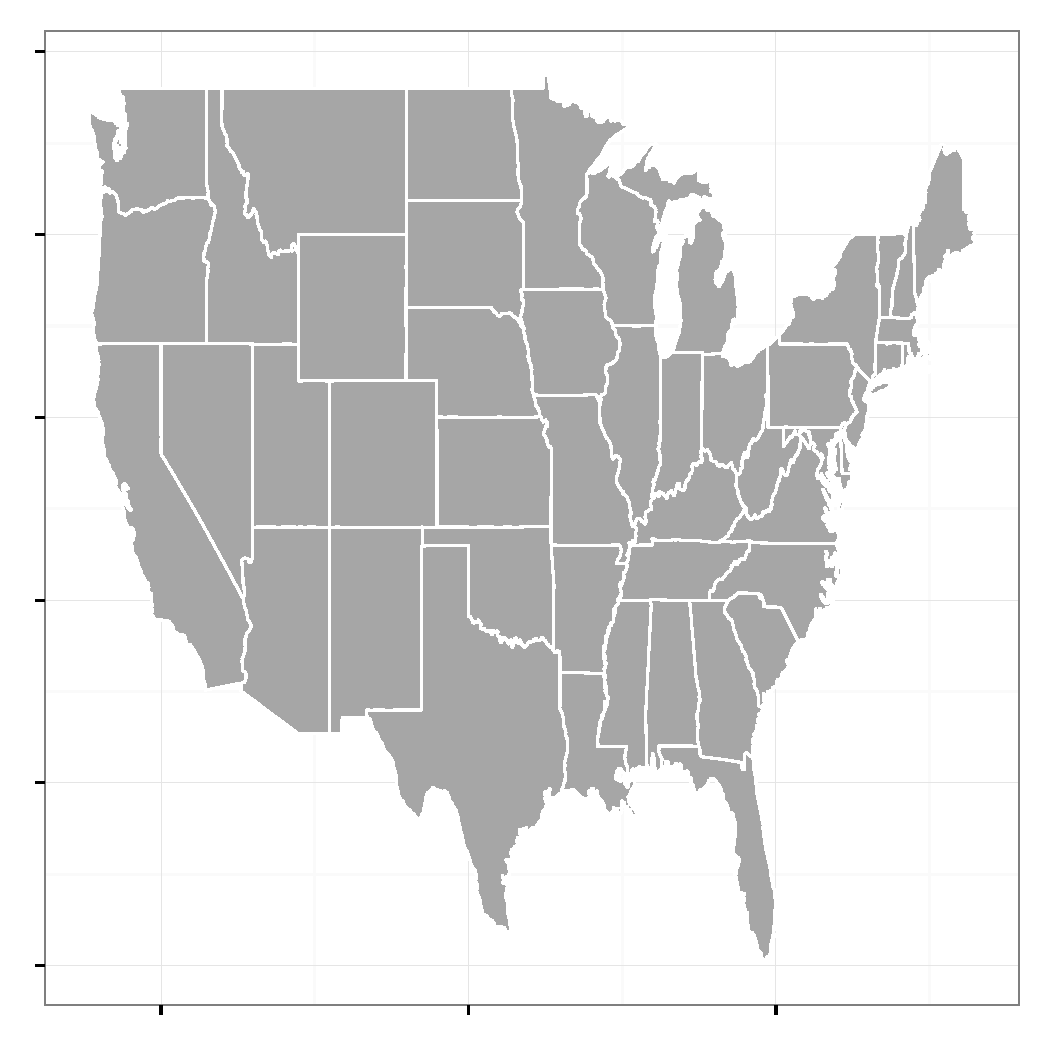
\includegraphics[width=\maxwidth]{./unnamed-chunk-11-1} 

}



\end{knitrout}
\newpage

We will now apply data collected from ESRI.  This data contains the longitude and latitude of each rail point.  These longitudes and latitudes will be used to visualize the main tracks used by railroad corporations. Again not the focus for now, but necessary in order to provide an understanding for the complexity of the network. \\

\begin{knitrout}
\definecolor{shadecolor}{rgb}{0.969, 0.969, 0.969}\color{fgcolor}\begin{kframe}
\begin{alltt}
\hlkwd{ggplot}\hlstd{()} \hlopt{+} \hlkwd{geom_polygon}\hlstd{(}\hlkwd{aes}\hlstd{(long,lat,} \hlkwc{group}\hlstd{=group),} \hlkwc{fill}\hlstd{=}\hlstr{"grey65"}\hlstd{,}
  \hlkwc{data}\hlstd{=ct.dat)} \hlopt{+} \hlkwd{geom_polygon}\hlstd{(}\hlkwd{aes}\hlstd{(long,lat,} \hlkwc{group}\hlstd{=group),}
  \hlkwc{color}\hlstd{=}\hlstr{'white'}\hlstd{,} \hlkwc{fill}\hlstd{=}\hlnum{NA}\hlstd{,} \hlkwc{data}\hlstd{=us.dat)} \hlopt{+} \hlkwd{theme_bw}\hlstd{()} \hlopt{+}
  \hlkwd{theme}\hlstd{(}\hlkwc{axis.text} \hlstd{=} \hlkwd{element_blank}\hlstd{(),} \hlkwc{axis.title}\hlstd{=}\hlkwd{element_blank}\hlstd{())} \hlopt{+}
  \hlkwd{geom_point}\hlstd{(}\hlkwc{colour}\hlstd{=}\hlstr{"grey50"}\hlstd{,}\hlkwc{data}\hlstd{=USTracks4,} \hlkwd{aes}\hlstd{(}\hlkwc{x}\hlstd{=coords.x1,}\hlkwc{y}\hlstd{=coords.x2,}\hlkwc{colour}\hlstd{=}\hlstr{"Rail"}\hlstd{),} \hlkwc{size} \hlstd{=} \hlnum{1}\hlstd{)}
\end{alltt}
\end{kframe}

{\centering \includegraphics[width=\maxwidth]{./unnamed-chunk-12-1} 

}



\end{knitrout}
\newpage

An overlayment of the drayage points were plotted as large points to mark the conveyance locations of the shipment. Notice, the Drayage included are all "major" access points into, out of, and all around the United States. This includes water access drayage and international, as they may be potential future clients. \\

\begin{knitrout}
\definecolor{shadecolor}{rgb}{0.969, 0.969, 0.969}\color{fgcolor}\begin{kframe}
\begin{alltt}
\hlkwd{ggplot}\hlstd{()} \hlopt{+} \hlkwd{geom_polygon}\hlstd{(}\hlkwd{aes}\hlstd{(long,lat,} \hlkwc{group}\hlstd{=group),} \hlkwc{fill}\hlstd{=}\hlstr{"grey65"}\hlstd{,}
  \hlkwc{data}\hlstd{=ct.dat)} \hlopt{+} \hlkwd{geom_polygon}\hlstd{(}\hlkwd{aes}\hlstd{(long,lat,} \hlkwc{group}\hlstd{=group),}
  \hlkwc{color}\hlstd{=}\hlstr{'white'}\hlstd{,} \hlkwc{fill}\hlstd{=}\hlnum{NA}\hlstd{,} \hlkwc{data}\hlstd{=us.dat)} \hlopt{+} \hlkwd{theme_bw}\hlstd{()} \hlopt{+}
  \hlkwd{theme}\hlstd{(}\hlkwc{axis.text} \hlstd{=} \hlkwd{element_blank}\hlstd{(),} \hlkwc{axis.title}\hlstd{=}\hlkwd{element_blank}\hlstd{())} \hlopt{+}
  \hlkwd{geom_point}\hlstd{(}\hlkwc{colour}\hlstd{=}\hlstr{"grey50"}\hlstd{,}\hlkwc{data}\hlstd{=USTracks4,} \hlkwd{aes}\hlstd{(}\hlkwc{x}\hlstd{=coords.x1,}\hlkwc{y}\hlstd{=coords.x2,}\hlkwc{colour}\hlstd{=}\hlstr{"Rail"}\hlstd{),} \hlkwc{size} \hlstd{=} \hlnum{1}\hlstd{)} \hlopt{+}
  \hlkwd{geom_point}\hlstd{(}\hlkwc{colour}\hlstd{=}\hlstr{"red"}\hlstd{,}\hlkwc{data}\hlstd{=Drayage,} \hlkwd{aes}\hlstd{(}\hlkwc{x}\hlstd{=lon,}\hlkwc{y}\hlstd{=lat,}\hlkwc{colour}\hlstd{=}\hlstr{"Drayage"}\hlstd{),}\hlkwc{size} \hlstd{=} \hlnum{4}\hlstd{)}
\end{alltt}
\end{kframe}

{\centering \includegraphics[width=\maxwidth]{./unnamed-chunk-13-1} 

}



\end{knitrout}
\newpage

Next intermodal corporation locations are plotted. \\

\begin{knitrout}
\definecolor{shadecolor}{rgb}{0.969, 0.969, 0.969}\color{fgcolor}\begin{kframe}
\begin{alltt}
\hlkwd{ggplot}\hlstd{()} \hlopt{+} \hlkwd{geom_polygon}\hlstd{(}\hlkwd{aes}\hlstd{(long,lat,} \hlkwc{group}\hlstd{=group),} \hlkwc{fill}\hlstd{=}\hlstr{"grey65"}\hlstd{,}
  \hlkwc{data}\hlstd{=ct.dat)} \hlopt{+} \hlkwd{geom_polygon}\hlstd{(}\hlkwd{aes}\hlstd{(long,lat,} \hlkwc{group}\hlstd{=group),}
  \hlkwc{color}\hlstd{=}\hlstr{'white'}\hlstd{,} \hlkwc{fill}\hlstd{=}\hlnum{NA}\hlstd{,} \hlkwc{data}\hlstd{=us.dat)} \hlopt{+} \hlkwd{theme_bw}\hlstd{()} \hlopt{+}
  \hlkwd{theme}\hlstd{(}\hlkwc{axis.text} \hlstd{=} \hlkwd{element_blank}\hlstd{(),} \hlkwc{axis.title}\hlstd{=}\hlkwd{element_blank}\hlstd{())} \hlopt{+}
  \hlkwd{geom_point}\hlstd{(}\hlkwc{colour}\hlstd{=}\hlstr{"grey50"}\hlstd{,}\hlkwc{data}\hlstd{=USTracks4,} \hlkwd{aes}\hlstd{(}\hlkwc{x}\hlstd{=coords.x1,}\hlkwc{y}\hlstd{=coords.x2,}\hlkwc{colour}\hlstd{=}\hlstr{"Rail"}\hlstd{),} \hlkwc{size} \hlstd{=} \hlnum{1}\hlstd{)} \hlopt{+}
  \hlkwd{geom_point}\hlstd{(}\hlkwc{colour}\hlstd{=}\hlstr{"red"}\hlstd{,}\hlkwc{data}\hlstd{=Drayage,} \hlkwd{aes}\hlstd{(}\hlkwc{x}\hlstd{=lon,}\hlkwc{y}\hlstd{=lat,}\hlkwc{colour}\hlstd{=}\hlstr{"Drayage"}\hlstd{),}\hlkwc{size} \hlstd{=} \hlnum{4}\hlstd{)} \hlopt{+}
  \hlkwd{geom_point}\hlstd{(}\hlkwc{colour}\hlstd{=}\hlstr{"yellow"}\hlstd{,}\hlkwc{data}\hlstd{=Customer4,} \hlkwd{aes}\hlstd{(}\hlkwc{x}\hlstd{=lon,}\hlkwc{y}\hlstd{=lat,}\hlkwc{colour}\hlstd{=}\hlstr{"City"}\hlstd{),}\hlkwc{size} \hlstd{=} \hlnum{2.2}\hlstd{)}
\end{alltt}
\end{kframe}

{\centering \includegraphics[width=\maxwidth]{./unnamed-chunk-14-1} 

}



\end{knitrout}
\newpage


There is no surprise as most of these corporations are located at major metropolitan areas, such as Chicago, New York, Los Angeles, and Minneapolis.

\begin{knitrout}
\definecolor{shadecolor}{rgb}{0.969, 0.969, 0.969}\color{fgcolor}\begin{kframe}
\begin{alltt}
\hlkwd{ggplot}\hlstd{()} \hlopt{+} \hlkwd{geom_polygon}\hlstd{(}\hlkwd{aes}\hlstd{(long,lat,} \hlkwc{group}\hlstd{=group),} \hlkwc{fill}\hlstd{=}\hlstr{"grey65"}\hlstd{,}
  \hlkwc{data}\hlstd{=ct.dat)} \hlopt{+} \hlkwd{geom_polygon}\hlstd{(}\hlkwd{aes}\hlstd{(long,lat,} \hlkwc{group}\hlstd{=group),}
  \hlkwc{color}\hlstd{=}\hlstr{'white'}\hlstd{,} \hlkwc{fill}\hlstd{=}\hlnum{NA}\hlstd{,} \hlkwc{data}\hlstd{=us.dat)} \hlopt{+} \hlkwd{theme_bw}\hlstd{()} \hlopt{+}
  \hlkwd{theme}\hlstd{(}\hlkwc{axis.text} \hlstd{=} \hlkwd{element_blank}\hlstd{(),} \hlkwc{axis.title}\hlstd{=}\hlkwd{element_blank}\hlstd{())} \hlopt{+}
  \hlkwd{geom_point}\hlstd{(}\hlkwc{colour}\hlstd{=}\hlstr{"grey50"}\hlstd{,}\hlkwc{data}\hlstd{=USTracks4,} \hlkwd{aes}\hlstd{(}\hlkwc{x}\hlstd{=coords.x1,}\hlkwc{y}\hlstd{=coords.x2,}\hlkwc{colour}\hlstd{=}\hlstr{"Rail"}\hlstd{),} \hlkwc{size} \hlstd{=} \hlnum{1}\hlstd{)} \hlopt{+}
  \hlkwd{geom_point}\hlstd{(}\hlkwc{data}\hlstd{=art.tot,} \hlkwd{aes}\hlstd{(}\hlkwc{x}\hlstd{=lon,}\hlkwc{y}\hlstd{=lat,}\hlkwc{colour}\hlstd{=din),}\hlkwc{size} \hlstd{=} \hlnum{4}\hlstd{)}
\end{alltt}
\end{kframe}

{\centering \includegraphics[width=\maxwidth]{./unnamed-chunk-15-1} 

}



\end{knitrout}


\begin{thebibliography}{9}

\bibitem{xtab}
    THIS IS NOT THE REAL ONE !!!!!!!!!!!!!!!!!!!!!!!!!!!!
    David B. Dahl,
    \emph{xtable: Export tables to LaTeX or HTML},
    R package version 1.7-3,
    http://CRAN.R-project.org/package=xtable, 
    2014

\bibitem{lamport94}
  Leslie Lamport, \emph{\LaTeX: A Document Preparation System}.
  Addison Wesley, Massachusetts,
  2nd Edition, 1994.

\bibitem{R-base}
  R Core Team, \emph{R: A Language and Environment for Statistical Computing},
  R Foundation for Statistical Computing,
  Vienna, Austria, http://www.R-project.org/ ,
  2014
  
\bibitem{R-knitr}
  Yihui Xie
  \emph{knitr: A general-purpose package for dynamic report generation in R},
  http://yihui.name/knitr/, 2014  

\end{thebibliography}

\end{document}

